\documentclass{beamer}
\usetheme{Madrid}

\usepackage{graphicx}
\graphicspath{{./img/}}

\AtBeginSection[]{
	\begin{frame}
		\frametitle{Table of Contents}
		\tableofcontents[currentsection]
	\end{frame}
}

\title{An agent-based model of military mechanization}
\subtitle{CSS 645}
\author{Tom Wallace}
\institute{George Mason University}
\date{Spring 2018}

\begin{document}

\frame{\titlepage}

\section{Background}

\begin{frame}
	\frametitle{Military mechanization}

	States differ in the composition of their militaries, particularly ground forces \\~\\

	One axis of comparison is \textbf{mechanization}
	\begin{itemize}
		\item \small The degree to which an army is comprised of infantry vs. ground combat vehicles \\~\\
	\end{itemize}

	Historical examples help illustrate the general idea
	\begin{itemize}
		\item \small 1970s Vietcong (low mechanization) vs. 1980s Israel (high mechanization)
		\item \small 1980s U.S. (higher mechanization) vs. present-day U.S. (lower mechanization)
	\end{itemize}
\end{frame}

\begin{frame}
	\frametitle{The consequences of choices regarding force structure are great}
	Academic and professional consensus that choices regarding military
	composition (including but not limited to mechanization) condition
	battlefield effectiveness \\~\\

	Size, cost, and complexity dictate that states can only slowly alter 
	military composition, even under great duress \\~\\

	``You go to war with the army you have'' \\~\\
\end{frame}

\begin{frame}
	\frametitle{The determinants of mechanization are disputed}
	One view stresses \textbf{security environment}: states adjust
	mechanization to be able to prevail in conflict
	\begin{itemize}
		\item \small Neighbors' and enemys' mechanization (e.g. 1930s
			France and Germany)
		\item \small Terrain (e.g. Switzerland)
		\item \small Insurgency (e.g. U.S.)\\~\\
	\end{itemize}

	Another view stresses \textbf{political, economic, and cultural
	factors}: states are not pure security-maximizers
	\begin{itemize}
		\item \small Regime type (e.g. democracy vs. autocracy)
		\item \small Economic endowments (e.g. capital vs. labor)
		\item \small Cultural norms (e.g. Irish tanks)\\~\\
	\end{itemize}

	Sechser and Saunders 2010 conclude the former matters much more than the
	latter
	\begin{itemize}
		\item \small Developed state-year level dataset on
			mechanization, 1979-2001
		\item \small Traditional longitudinal data analysis (OLS)
	\end{itemize}

\end{frame}

\begin{frame}
	\frametitle{Viewing their findings through an ABM lens}

	Emphasis on \textbf{spatiality}: what are my neighbors doing? \\~\\

	My actions affect your actions affect my actions... $\to$ \textbf{positive feedback loops} \\~\\

	Estimated statistical coefficients implicitly claim particular cognitive model
	\begin{itemize}
		\item \small If neighbors mechanization goes up by $X$, I raise my mechanization by $\beta$ \\~\\
	\end{itemize}

	My research question: do their findings hold up under an ABM formulation?
\end{frame}

\section{Model Description}

\begin{frame}
	\frametitle{Agents}
	Agent = state actor \\~\\

	Covers all countries in the world, minus microstates and ``inheritance'' problem

	\begin{figure}[h!]
		\centering
		\caption{Agents}
		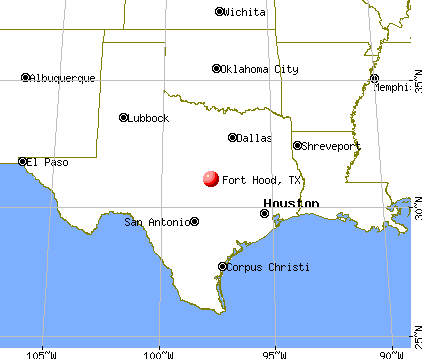
\includegraphics[scale=0.04]{map.png}
	\end{figure}
\end{frame}

\begin{frame}
	\frametitle{Agent attributes}
	\begin{table}[h]
		\centering
		\begin{tabular}{|l l|}
			\hline
			\textbf{Identity} & \textit{Name} \\
			& \\
			\textbf{Mechanization} & \textit{Mechanization} \\
			& \\
			\textbf{Spatiality} & \textit{Neighbors} \\
			& \\
			\textbf{Inter-agent Relationships} & \textit{Enemies} \\
			& \\
			\textbf{Perception} & \textit{EnemiesMech} \\
			& \textit{NeighborsMech} \\
			& \textit{Lesson} \\
			& \\
			\textbf{Cognition} & \textit{EnemyMechSensitivity} \\
			& \textit{NeighborsMechSensitivity} \\
			& \textit{LessonSensitivity} \\
			\hline
		\end{tabular}
	\end{table}
\end{frame}

\begin{frame}
	\frametitle{Additional notes on agents and environment}
	Mechanization: combat vehicles per 100 infantry (data: IISS)\\~\\

	Spatiality: neighbor relationships rather than full-blown GIS \\~\\

	Enemies: defined on 10-year Militarized Interstate Dispute (MID) history\\~\\

	Perception: every time step, agents observe behavior of others and respond\\~\\

	Cognition: adjust own mechanization level based on neighbors, enemies, defeat in counter-insurgency
	\begin{itemize}
		\item \small Cognition is heterogenous across agents:
			coefficients drawn from distributions of Sechser and
			Saunders 
		\item \small Update equation:
			\begin{multline}
				\textrm{Mech}_i^{(t+1)} = \textrm{Mech}_i^{(t)}
				+ (\textrm{NeighborMechSensitivity}_i \times \textrm{NeighborMech}_i^{(t)}) \\
				+ (\textrm{EnemyMechSensitivity}_i \times \textrm{EnemyMech}_i^{(t)}) \\
				+ (\textrm{LessonSensitivity}_i \times I_{\textrm{Lesson}}(t, i))
			\end{multline}
	\end{itemize}
\end{frame}

\begin{frame}
	\frametitle{Time}
	Initialized in 1979, proceeds in two-year timesteps until 2001 \\~\\

	Every turn, agents (in random activation order):
	\begin{itemize}
		\item \small Perceive world
		\item \small Update assessment of neighbors, enemies, AML
		\item \small Adjust own mechanization \\~\\
	\end{itemize}

	Because agent cognition has random element, model is stochastic and must
	be run many times \\~\\

	General research strategy: initialize with values from 1979, run, see if model results in 2001 match reality at both
	actor- and system-level
\end{frame}

\section{Findings}

\begin{frame}
	\frametitle{Model mechanization much higher at system-level than
	occurred in reality}
\begin{table}[h]
	\centering
	\caption{Comparison}
	\begin{tabular}{|l r r|}
		\hline
		\textbf{Year} & \textbf{Model} & \textbf{Reality} \\
		1979 & 0.0156 & 0.0139 \\
		1981 & 0.0189 & 0.0167 \\
		1983 & 0.0229 & 0.0167 \\
		1985 & 0.0280 & 0.0183 \\
		1987 & 0.0351 & 0.0187 \\
		1989 & 0.0415 & 0.0197 \\
		1991 & 0.0512 & 0.0215 \\
		1993 & 0.0636 & 0.0229 \\
		1995 & 0.0804 & 0.0231 \\
		1997 & 0.1014 & 0.0270 \\
		1999 & 0.1319 & 0.0272 \\
		2001 & 0.1730 & 0.0291 \\
		\hline
	\end{tabular}
\end{table}
\end{frame}

\begin{frame}
	\frametitle{Mechanization not uniform across agents - actually
	\textit{lower} in some}
	\begin{table}[h]
		\centering
		\caption{Mexico}
		\begin{tabular}{|l r r|}
			\hline
			\textbf{Year} & \textbf{Model} & \textbf{Reality} \\
			1979 & 0.0013 & 0.0012 \\
			1981 & 0.0014 & 0.0012 \\
			1983 & 0.0018 & 0.0026 \\
			1985 & 0.0019 & 0.0013 \\
			1987 & 0.0021 & 0.0019 \\
			1989 & 0.0022 & 0.0027 \\
			1991 & 0.0024 & 0.0030 \\
			1993 & 0.0026 & 0.0033 \\
			1995 & 0.0030 & 0.0035 \\
			1997 & 0.0032 & 0.0074 \\
			1999 & 0.0036 & 0.0082 \\
			2001 & 0.0040 & 0.0075 \\
			\hline
		\end{tabular}
	\end{table}
\end{frame}

\begin{frame}
	\frametitle{Findings driven by few outliers}
	\begin{table}[h]
		\centering
		\caption{Highest mechanization scores, 2001}
		\begin{tabular}{|l r|}
			\hline
			\textbf{Agent} & \textbf{Mechanization Score} \\
			Israel & 1.59 \\
			USA & 1.34 \\
			Kuwait & 1.14 \\
			Russia & 1.06 \\
			\hline
		\end{tabular}
	\end{table}
\end{frame}

\begin{frame}
	\frametitle{Outliers are clustered by neighborhood and relationship}
	\begin{table}[h]
		\centering
		\caption{Top 20 mechanized agents at simulation end, by region}
		\begin{tabular}{|l l l l l l|}
			\hline
			\textbf{MENA} & \textbf{Europe \& FSU} & \textbf{Africa} & \textbf{Americas} & \textbf{Asia} & \textbf{Oceania} \\
			Israel       & Russia         & Sudan        & USA    & (none) & (none) \\
			Kuwait       & France         & S. Africa    & Canada &        &        \\
			Iran         & UK             &              &        &        &        \\
			Libya        & Greece         &              &        &        &        \\
			Iraq         & Netherlands    &              &        &        &        \\
			Syria        & Poland         &              &        &        &        \\
			KSA          &                &              &        &        &        \\
			Egypt        &                &              &        &        &        \\
			Lebanon      &                &              &        &        &        \\
			Turkey       &                &              &        &        &        \\
			\hline
		\end{tabular}
	\end{table}
\end{frame}

\section{Discussion}

\begin{frame}
	\frametitle{Findings driven by positive feedback loop}

	State A raises mechanization, which causes neighbor / enemy State B to
	increase own mechanization... (\textit{security dilemma})\\~\\

	States with high exposure to this feedback loop due to many enemies and
	neighbors become outliers \\~\\

	Positive feedback loops are hallmark of complex system
	\begin{itemize}
		\item \small Autonomous, cognitive, heterogenous agents
		\item \small Spatiality
		\item \small Interaction
	\end{itemize}
\end{frame}

\begin{frame}
	\frametitle{Implications for larger literature}
	Findings imply orthodox, security environment-centric, ``external'' view
	is incomplete: there must be some variable or set of variables acting as
	a ``brake'' on military mechanization to mitigate the aforementioned
	positive feedback loop \\~\\

	Model cannot say exactly what those missing variables (but could assess
	whether candidates ``work'' in simulation...hint hint) \\~\\

	Agent-based models relatively rare in international relations (e.g.
	Cederman 1997, Axelrod 1997)
\end{frame}
\begin{frame}
	\frametitle{Larger course themes}
	
	Analyzed-analyzed\\~\\
	
	Empirical methods and validation central to research strategy \\~\\

	GIS in ABM: what level of detail is good enough? \\~\\

	Understanding behavior of complex models \\~\\

\end{frame}

\end{document}
